\documentclass[tikz, border=3mm]{standalone}
\usepackage{tikz}
\usetikzlibrary{
    arrows.meta,         % For arrow tips
    decorations.markings,% For placing arrows along paths
    patterns.meta,       % For hatching patterns
    calc,                % For coordinate calculations (optional here, but good practice)
    positioning          % For label positioning
}

\begin{document}
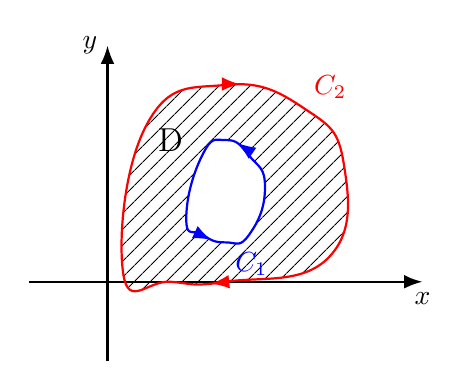
\begin{tikzpicture}[
    >=Latex, % Set default arrow tip style
    axis/.style={->, thick}, % Style for axes
    blob/.style={thick},     % Base style for blob borders
    % Arrow styles using decorations
    ccw_arrows/.style={postaction={decorate, decoration={markings,
        % Place multiple arrows CCW
        mark=at position 0.15 with {\arrow[#1, thick]{>}}, % Use color argument #1
        mark=at position 0.65 with {\arrow[#1, thick]{>}}
    }}},
    cw_arrows/.style={postaction={decorate, decoration={markings,
        % Place multiple arrows CW (reversed on path)
        mark=at position 0.15 with {\arrowreversed[#1, thick]{>}}, % Use color argument #1
        mark=at position 0.65 with {\arrowreversed[#1, thick]{>}}
    }}},
    hatchstyle/.style={pattern={Lines[angle=45, distance=4pt, line width=0.4pt]}, pattern color=black} % Hatching style
]

    % Define coordinates for blobs (adjust coordinates & tension for desired shape)
    \def\coordsTwo{(0.2, 0.1) (0.5, 2.0) (1.5, 2.5) (2.5, 2.2) (3.0, 1.5) (2.8, 0.3) (1.5, 0.0) (0.8, 0.0)}
    \def\coordsOne{(1.0, 0.8) (1.2, 1.6) (1.5, 1.8) (1.8, 1.6) (2.0, 1.2) (1.8, 0.6) (1.5, 0.5) (1.2, 0.6)}

    % Axes
    \draw[axis] (-1, 0) -- (4, 0) node[below] {$x$};
    \draw[axis] (0, -1) -- (0, 3) node[left] {$y$};

    % --- Layered Fill (Replaces Clipping) ---
    % Layer 1: Fill outer blob with hatch pattern
    \fill[hatchstyle] plot[smooth cycle, tension=0.8] coordinates {\coordsTwo};

    % Layer 2: Fill inner blob with white (background color) to erase hatch
    \fill[white] plot[smooth cycle, tension=0.9] coordinates {\coordsOne};
    % --- End Layered Fill ---

    % --- Draw Blob Borders with Arrows (Draw AFTER fills) ---
    % Outer Blob C2 (Red, CCW)
    \draw[blob, red, ccw_arrows={red}] plot [smooth cycle, tension=0.8] coordinates {\coordsTwo};
    \node[red, above right] at (2.5, 2.2) {$C_2$}; % Label C2

    % Inner Blob C1 (Blue, CW)
    \draw[blob, blue, cw_arrows={blue}] plot [smooth cycle, tension=0.9] coordinates {\coordsOne};
    \node[blue, below right] at (1.5, 0.5) {$C_1$}; % Label C1

    % Label Region D
    \node[font=\large] at (0.8, 1.8) {D}; % Place D in shaded area

\end{tikzpicture}
\end{document}